\subsection[BDI in AgentSpeak(L) and Jason]{BDI in AgentSpeak(L) and Jason$^{\blacktriangle,\circ}$}
AgentSpeak(L) is an agent-oriented programming language which taking the inspiration from the work on the BDI model and BDI implementations~\cite{rafael_BDIAgent_2005}.
This language is based on a restricted first-order language with events and actions~\cite{anand_AgentSpeak_1996}.
The behaviour of an agent such as the interaction of that agent with the environment is implemented in AgentSpeak(L).
In other words, AgentSpeak(L) encodes beliefs, desires, and intentions in a way processable by an agent.
This section presents the interpretation cycle of an AgentSpeak(L) program as implemented in Jason.
It shows a more extensive picture on the reasoning process of a Jason BDI agent.

As explained by Rao~\cite{anand_AgentSpeak_1996} beliefs model the current state of an agent, expressing its knowledge.
They may be modified on environment changes due to some internal or external events.
Rao furthermore describes states the agent wants to reach are desires as in the earlier presented BDI approach.
Analogously, he continues to define intentions as an agent's attempt to reach such a state by the commitment to concrete plans.

As Jason is an interpreter for AgentSpeak(L) with Java-base extensions~\cite{rafael_Javabased}, it becomes practically suitable for multi-agent systems.
Some details on the functioning of an AgentSpeak(L) interpreter are presented in \autoref{fig:ASL_interpreter}.
\begin{figure}[h]
  \centering
  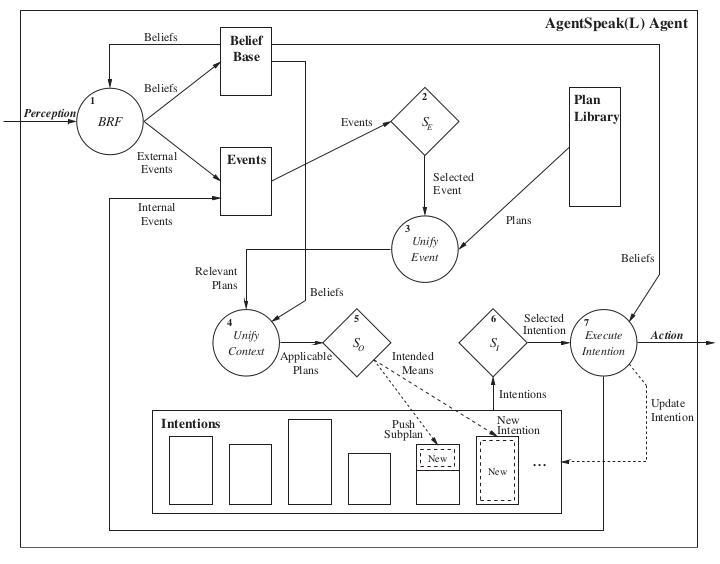
\includegraphics[width=\textwidth]{images/BDI_ASL_interpreter}
  \caption{An interpretation cycle of an AgentSpeak(L) program~\cite{rafael_BDIAgent_2005}.}
  \label{fig:ASL_interpreter}
\end{figure}

An AgentSpeak(L) agent consists of its initial knowledge which is encoded in its belief and a plan library~\cite{rafael_BDIAgent_2005}.
\autoref{fig:ASL_interpreter} does not visualise the source of the beliefs in the belief base properly.
The beliefs do not only come from external perceptions of the environment. % TODO we could improve that graphic by adding this
Instead, they can also be the result of plan executions by the agents which only have internal effects.
The beliefs from perceptions are annotated by \texttt{source(percept)}.
In our implementation, there are $34$ perceptions received from the server, which an agent would store as a belief.
Initial beliefs and generally all internal beliefs are annotated with \texttt{source(self)}.
The external beliefs describe the current states of each agent such as its energy or its role.
These beliefs are not immutable and can be used and modified in plans.

In the interpretation cycle shows that events also play an important role.
After the selection of the events by the \emph{event selection function} $\mathcal{S_E}$ the events will be unified with the triggering events in the head of the plans from the plan library.
In our system, there are $184$ plans in total.
We have $88$ plans with discrete triggering events meaning that our own plans handle $88$ different events.

Desires in AgentSpeak(L) are expressed through test or achievement goals.
We explicitly implemented achievement goals in our program.
For example, \texttt{!doParry} is an achievement goal that will lead to the execution of the \texttt{parry} action when a certain plan matches the event.
However, querying the belief base in the context of a plan is converted by Jason into an achievement goal automatically.

For some tasks, we have multiple plans as there are many different contexts to consider.
As an example, attacking is covered in more plans as the strategy is complex.
A variety of situations must be considered before attacking like determining if there is an enemy nearby, if the agent should move towards the enemy, if it has enough energy, what to do if there is no enemy and so on.
Similarly, $31$ percent of all plans are associated with building zones.
The reason for this is mainly due to the complexity of communication between agents and many special cases to consider.
On the other hand, other actions do not need excessive planning like the \texttt{buy} action.
When the specified Saboteur agent does not see any enemy agents nearby, it will upgrade its visibility range and health without considering more than just its energy and the available money.
\autoref{fig:plan_allocation} illustrates the amount of plans used for different actions.
\begin{figure}
  \centering
  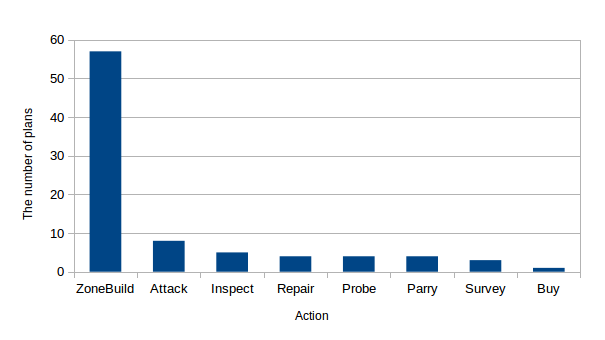
\includegraphics[width=\textwidth]{images/BDI_plan_distribution_action}
  \caption{Plan distribution for actions.}
  \label{fig:plan_allocation}
\end{figure}
Similarly, the amount of plans executable only if the agent has a particular role vary a lot.
\autoref{fig:baselinex} illustrates this and shows that the Saboteur agent had more role-specific plans than e.g.\ for the Sentinel agent.
The reason for this is that we have a complex, offensive strategy for our Saboteur agents but there are not even Sentinel-exclusive actions.
This figure does not count plans executable by all roles such as going to another vertex.
\begin{figure}
  \centering
  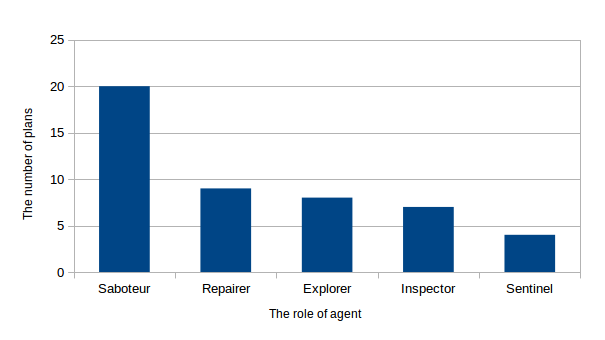
\includegraphics[width=\textwidth]{images/BDI_plan_distribution_role}
  \caption{Plan distribution for agents.}
  \label{fig:baselinex}
\end{figure}

All those plans are loaded into the plan library.
To determine when which plan is actually applicable, the \emph{option selection function} $\mathcal{S_O}$ is needed.
It receives the plans whose triggering event matches matched against the belief base.
This ensures that it only reasons about plans which are executable in the current situation by inspecting their context.
As a result, $\mathcal{S_O}$ draws an applicable plan for an intention.
The plans for the intentions are stored with new plans creating a new intention.
Subgoals, triggered from other plans, are added to existing intentions.
As the drawn plans match the contexts, they can be seen as partially instantiated~\cite{rafel_Javabased_2007}.

Beliefs, desires and intentions are introduced above, but many agent languages contain all these three.
One of the reasons to choose Jason as programming language was that Jason provides an already implemented set of internal actions and is extensible by user-defined internal actions, which are programmed in Java~\cite{rafael_Javabased_2007}.
Besides the original internal actions like \texttt{.print} or \texttt{.send}, we developed $32$ internal actions.
Most of these internal actions are devoted to receiving information about the map, such as finding high value vertices.
They hence do not play a big part in our development from a BDI perspective.

This section gave a more in-depth overview of the reasoning in Jason in the context of the BDI model.
Jason's and AgentSpeak(L)'s implementation of the BDI agent architecture manage to close the gap between the theoretic model and a practically suitable language for multi-agent development.
Nevertheless, we faced several problems during implementation which are further discussed in \autoref{con:learned}.
